\documentclass[10pt]{beamer}

\usepackage[T2A]{fontenc}
\usepackage[utf8]{inputenc}
\usepackage[russian,english]{babel}

\usefonttheme[onlymath]{serif}

\usetheme[progressbar=frametitle]{metropolis}
\usepackage{appendixnumberbeamer}

\usepackage{booktabs}
\usepackage[scale=2]{ccicons}

\usepackage{pgfplots}
\usepgfplotslibrary{dateplot}

\usepackage{xspace}
\newcommand{\themename}{\textbf{\textsc{metropolis}}\xspace}
\newcommand{\TODO}[1]{\textbf{\textcolor{red}{TODO: #1}}}

\date{}
\author{Екатерина Тузова}


\title{Лекция 3}
\subtitle{Кластеризация}

\begin{document}

\maketitle

\section{Разбор летучки}

\section{Мотивирующий пример}

\begin{frame}{Постановка задачи кластеризации}
  Кластеризация -- задача разделения объектов одной природы на несколько групп так, чтобы объекты в одной группе обладали одним и тем же свойством.\\
  \bigbreak
  Кластеризация -- это обучение без учителя.
\end{frame}

\begin{frame}{Постановка задачи кластеризации}
	$X$ -- пространство объектов\\
	$\rho: X \times X \rightarrow [0, \infty)$ -- функция расстояния между объектами\\
	\bigbreak
	\alert{Найти}:\\
	$Y$ -- множество кластеров \\
	$a: X \rightarrow Y$ -- алгоритм кластеризации
\end{frame}


\section{Степени свободы в постановке задачи}

\begin{frame}{Степени свободы в постановке задачи}
	\begin{itemize} [<+- | alert@+>]
		\item[--] Критерий качества кластеризации
		\item[--] Число кластеров неизвестно заранее
		\item[--] Результат кластеризации существенно зависит от метрики
	\end{itemize}
\end{frame}

\section{Цели кластеризации}

\begin{frame}{Цели кластеризации}
	\begin{itemize} [<+- | alert@+>]
		\item[--] Сократить объём хранимых данных
		\item[--] Выделить нетипичные объекты
		\item[--] Упростить дальнейшую обработку данных
		\item[--] Построить иерархию множества объектов				
	\end{itemize}
\end{frame}

\section{Какие бывают кластеры?}

\begin{frame}{Сгущения}
	\begin{center}
    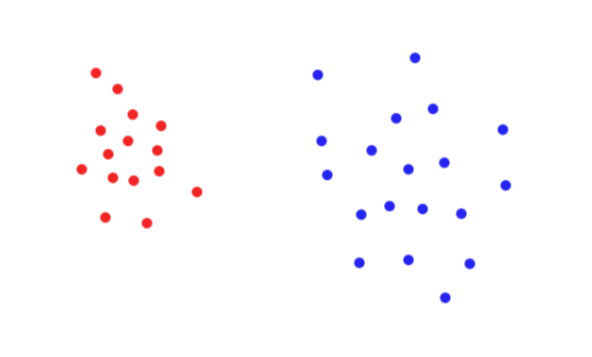
\includegraphics[height=0.8 \textheight, keepaspectratio = true]{images/cluster1}  
	\end{center}
\end{frame}


\begin{frame}{Ленты}
	\begin{center}
	  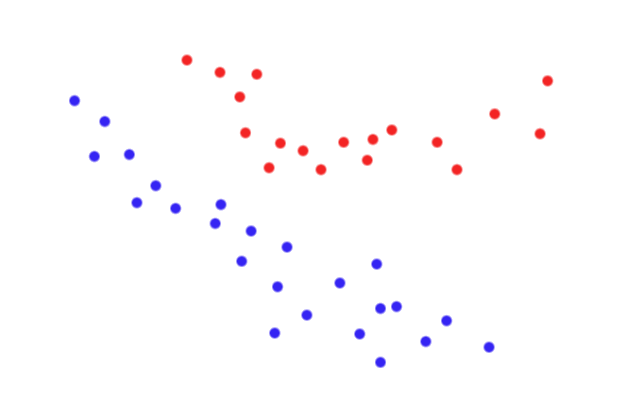
\includegraphics[height=0.8 \textheight, keepaspectratio = true]{images/cluster2}  
	\end{center}
\end{frame}

\begin{frame}{С центром}
	\begin{center}
	  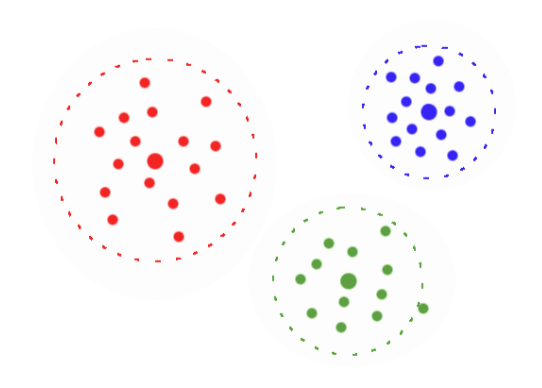
\includegraphics[height=0.8 \textheight, keepaspectratio = true]{images/cluster3}  
	\end{center}
\end{frame}

\begin{frame}{С перемычками}
	\begin{center}
	  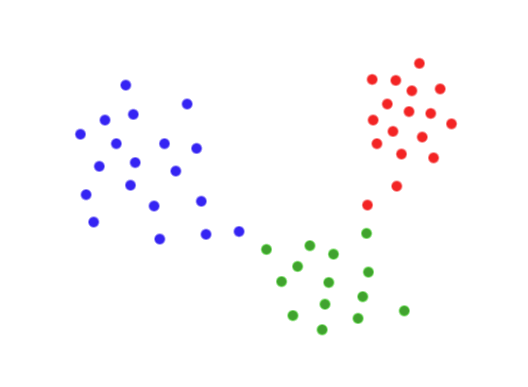
\includegraphics[height=0.8 \textheight, keepaspectratio = true]{images/cluster4}  
	\end{center}
\end{frame}

\begin{frame}{На фоне}
	\begin{center}
	  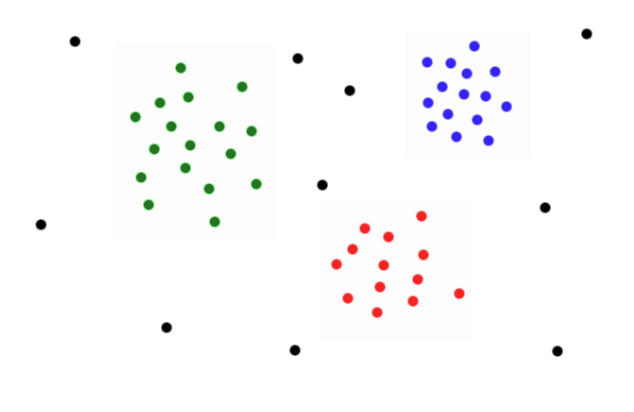
\includegraphics[height=0.8 \textheight, keepaspectratio = true]{images/cluster5}  
	\end{center}
\end{frame}

\begin{frame}{Перекрывающиеся}
	\begin{center}
	  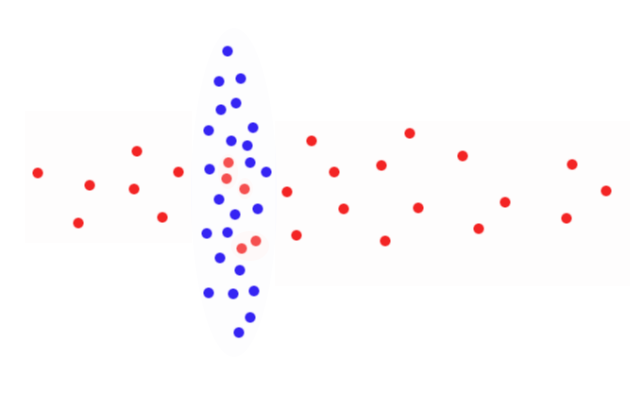
\includegraphics[height=0.8 \textheight, keepaspectratio = true]{images/cluster6}  
	\end{center}
\end{frame}

\begin{frame}{Чувствительность к выбору метрики}
  \TODO{пример из нашего датасета}
\end{frame}

\section{Оценка качества кластеризации}

\begin{frame}{Оценка качества кластеризации}
  \alert{Идея}: Минимизировать среднее внутрикластерное расстояние и при этом максимизировать среднее межкластерное расстояние.
\end{frame}

\begin{frame}{Оценка качества кластеризации}
  \alert{Идея}: Минимизировать среднее внутрикластерное расстояние и при этом максимизировать среднее межкластерное расстояние.
	\bigbreak
	$${\frac{\sum\limits_{a(x_i) = a(x_j)} \rho(x_i, x_j)}{\sum\limits_{a(x_i) = a(x_j)} 1} \rightarrow \min}$$
	\bigbreak
	$${\frac{\sum\limits_{a(x_i) \neq a(x_j)} \rho(x_i, x_j)}{\sum\limits_{a(x_i) \neq a(x_j)} 1} \rightarrow \max}$$
\end{frame}


\begin{frame}{Методы кластеризации}
	\begin{enumerate} [-]
		\item Иерархические
		\item Графовые 
		\item Статистические 
	\end{enumerate}
\end{frame}

\section{Иерархическая кластеризация}

\begin{frame}{Агломеративный алгоритм Ланса-Уильямса}
	\alert{Идея}:\\
	\begin{enumerate}
		\item Считаем каждую точку кластером. 
		\item Затем объединяем ближайшие точки в новый кластер. 
		\item Повторяем.
	\end{enumerate}
\end{frame}


\begin{frame}{Алгоритм Ланса-Уильямса}
	${C_1 = \left\{ \left\{ x_1\right\}, \left\{x_2 \right\}, \dots, \left\{x_l \right\} \right\}}$\\
	for ${t=2, \dots, l }$:\\
	\hspace{5mm} ${(U, V) = \arg\min\limits_{U \neq V} \rho(U, V)}$\\
	\hspace{5mm} $W = U \cup V$\\
	\hspace{5mm} ${C_t = C_{t-1} \cup \left\{ W \right\}\setminus \left\{U, V \right\} }$\\
	\hspace{5mm} foreach ${S \in C_t}$\\
	\hspace{10mm}   вычислить $\rho(W, S)$\\
\end{frame}


\begin{frame}{Алгоритм Ланса-Уильямса}
  Чего не хватает?
\end{frame}

\begin{frame}{Формула Ланса-Уильямса}
	\begin{minipage}[t]{0.55\linewidth}
		Расстояние $\rho(W, S)$?\\
		${ W = \left\{ U \cup V \right\} }$\\	
		Знаем:\\
		${\rho(U, S), \rho(V, S), \rho(U, V)}$
	\end{minipage}%

\TODO{картинка}
%	\begin{minipage}[t]{0.45\linewidth}
%	    \begin{figure}[htbp]
%			  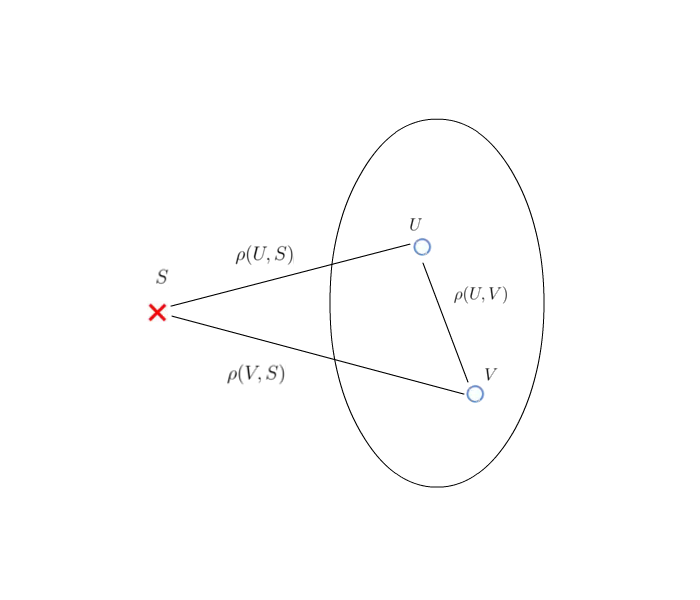
\includegraphics[height=130pt, keepaspectratio = true]{images/lans-formula}  
%			\end{figure}
%	\end{minipage}%
\end{frame}

\begin{frame}{Формула Ланса-Уильямса}
	Расстояние $\rho(W, S)$?\\
	${ W = \left\{ U \cup V \right\} }$\\
	\bigbreak
	Знаем:\\
	${\rho(U, S), \rho(V, S), \rho(U, V)}$\\
  \bigbreak
	${\rho(U \cup V, S) = \alpha_U \rho(U, S) + \alpha_V \rho(V, S) + }$ \\
	\hspace{30mm} ${ + \beta \rho(U, V) + \gamma \vert \rho(U, S) - \rho(V, S)\vert}$\\
	\bigbreak
	${\alpha_U, \alpha_V, \beta, \gamma}$ -- числовые параметры
\end{frame}

\begin{frame}{Параметры}
	Значения параметров
	${\alpha_U, \alpha_V, \beta, \gamma}$ ?
\end{frame}

\begin{frame}{Расстояние ближнего соседа}
	\TODO{картинка}
%	\begin{figure}[htbp]
%	  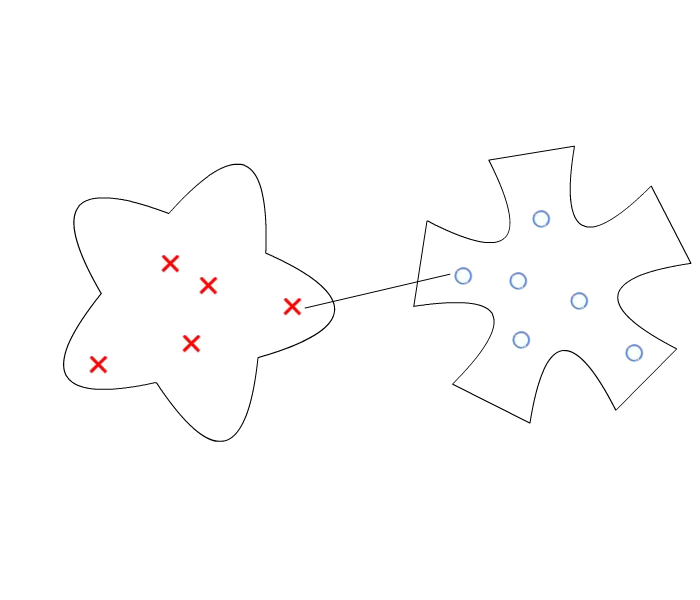
\includegraphics[height=100pt, keepaspectratio = true]{images/lans1}  
%	\end{figure}
\end{frame}

\begin{frame}{Расстояние ближнего соседа}
	Расстояние ближнего соседа:\\
	\TODO{картинка}
%	\begin{figure}[htbp]
%	  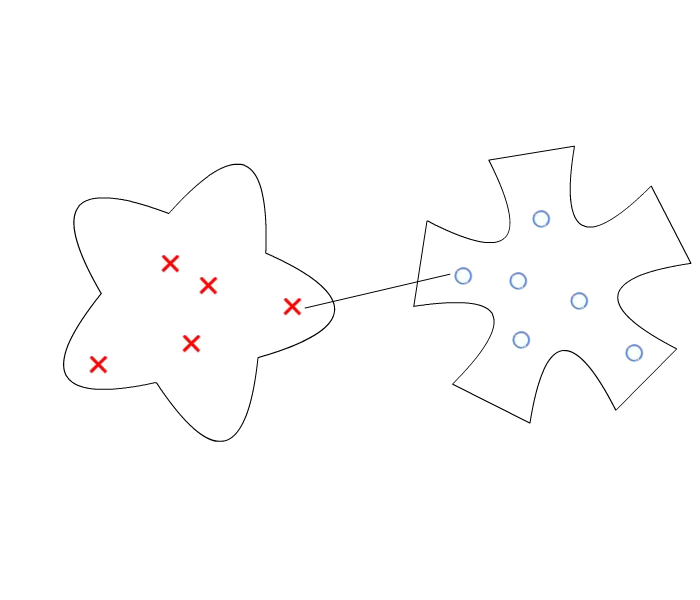
\includegraphics[height=100pt, keepaspectratio = true]{images/lans1}  
%	\end{figure}
	${\alpha_U = \alpha_V = \frac{1}{2}}$ \\${\beta = 0}$ \\${\gamma = -\frac{1}{2}}$
\end{frame}

\begin{frame}{Расстояние дальнего соседа}
	Расстояние дальнего соседа:\\
  \TODO{картинка}
%	\begin{figure}[htbp]
%	  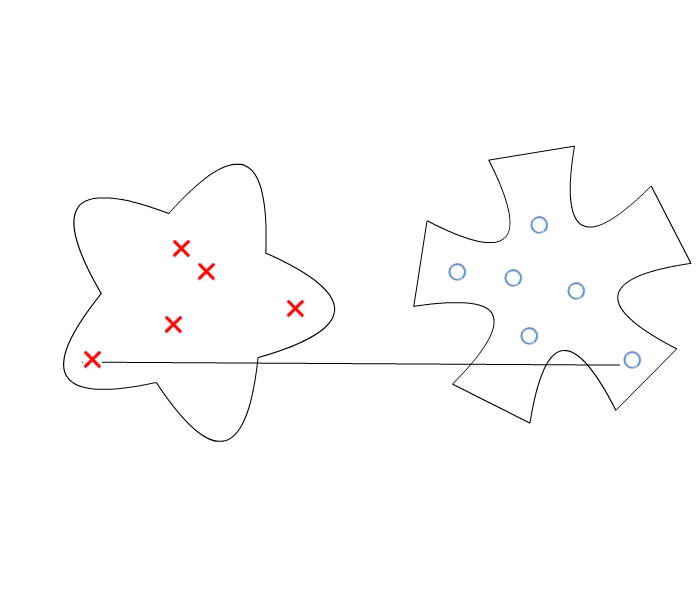
\includegraphics[height=100pt, keepaspectratio = true]{images/lans2}  
%	\end{figure}
\end{frame}

\begin{frame}{Расстояние дальнего соседа}
	\TODO{картинка}
%	\begin{figure}[htbp]
%	  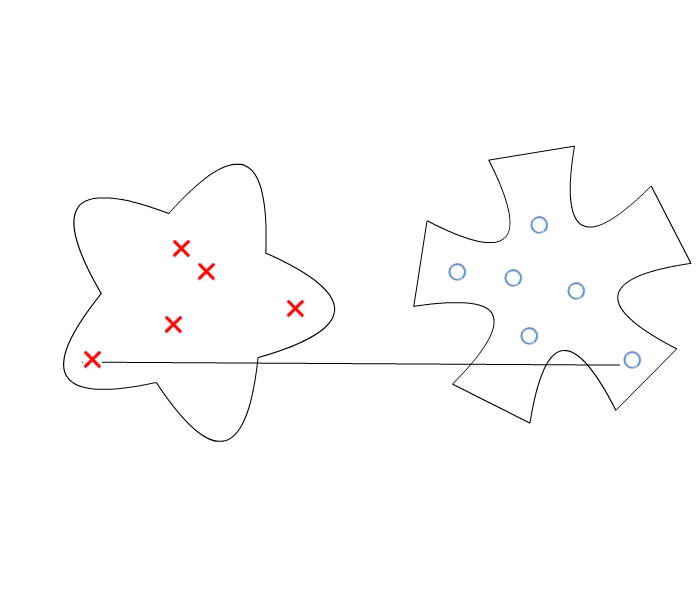
\includegraphics[height=100pt, keepaspectratio = true]{images/lans2}  
%	\end{figure}
	${\alpha_U = \alpha_V = \frac{1}{2}}$ \\${\beta = 0}$ \\${\gamma = \frac{1}{2}}$
\end{frame}

\begin{frame}{Групповое среднее}
  \TODO{картинка}
%	\begin{figure}[htbp]
%	  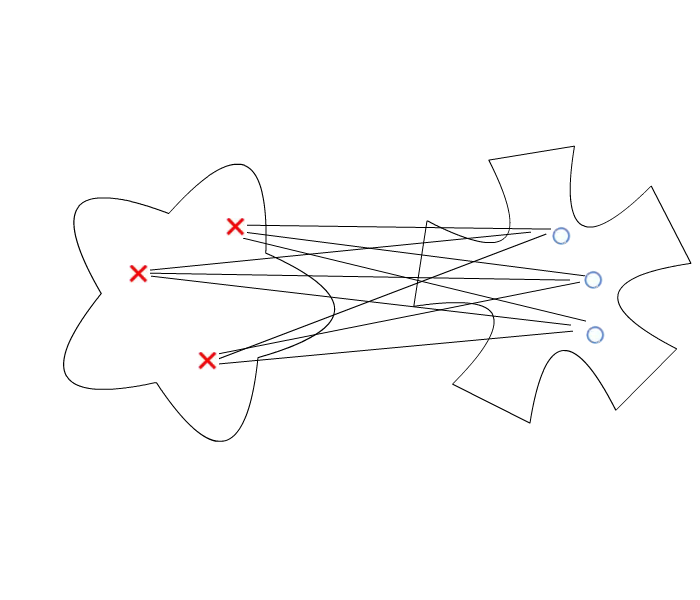
\includegraphics[height=100pt, keepaspectratio = true]{images/lans3}  
%	\end{figure}
\end{frame}

\begin{frame}{Групповое среднее}
  \TODO{картинка}
%	\begin{figure}[htbp]
%	  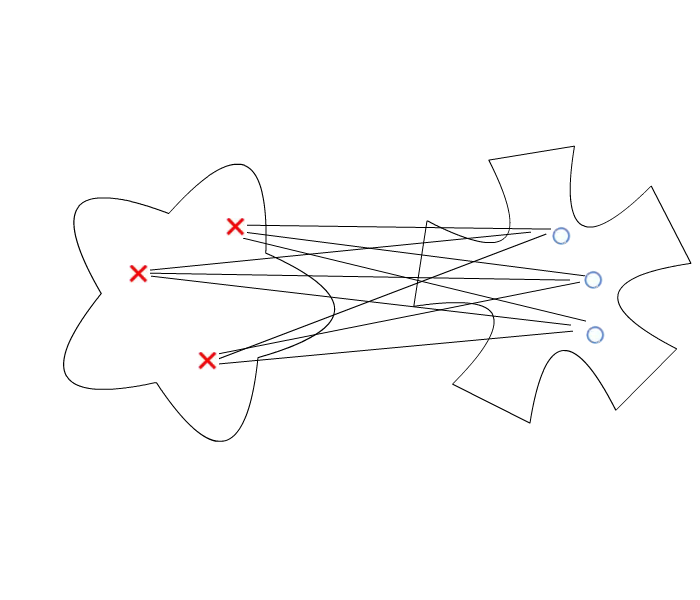
\includegraphics[height=100pt, keepaspectratio = true]{images/lans3}  
%	\end{figure}
	${\alpha_U = \frac{\vert U \vert}{\vert W \vert}}$\\${\alpha_V = \frac{\vert V \vert}{\vert W \vert}}$ \\${\beta = \gamma = 0}$
\end{frame}

\begin{frame}{Расстояние Уорда}
  \TODO{картинка}
%	\begin{figure}[htbp]
%	  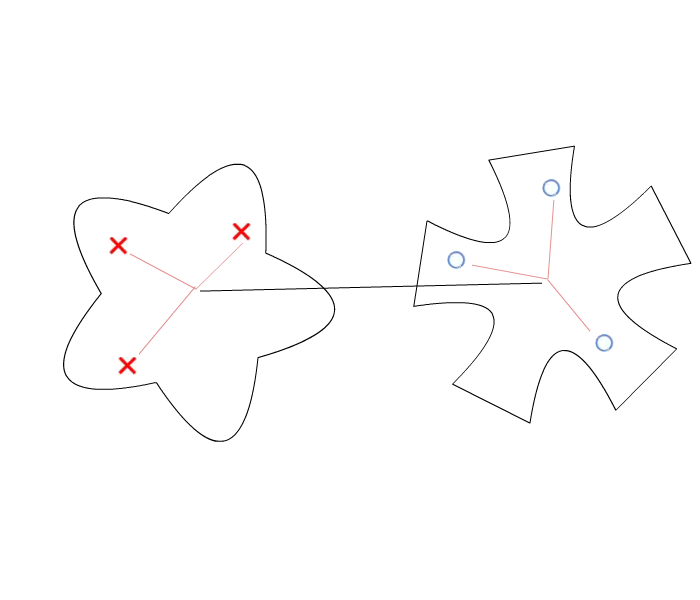
\includegraphics[height=100pt, keepaspectratio = true]{images/lans4}  
%	\end{figure}

  ${\alpha_U = \frac{\vert S \vert + \vert U \vert}{\vert S \vert + \vert W \vert}}$\\${\alpha_V = \frac{\vert S \vert + \vert V \vert}{\vert S \vert + \vert W \vert}}$ \\${\beta = \frac{ -\vert S \vert}{\vert S \vert + \vert W \vert}}$ \\${\gamma = 0}$
\end{frame}

\section{Визуализация кластеров}

\begin{frame}{Диаграмма вложения}
  \TODO{картинка}  
\end{frame}

\begin{frame}{Дендрограмма}
  \TODO{картинка}  
\end{frame}


\begin{frame}{Вопрос}
  \centering  
  Может ли так случиться, что дендрограмма имеет самопересечения?
\end{frame}

\begin{frame}{Свойство монотонности}
  Кластеризация монотонна, если на каждом шаге расстояние $\rho$ между объединяемыми кластерами не уменьшается.\\
  $\rho_2 \leq \rho_3 \leq \dots \leq \rho_l$
\end{frame}

\section{Графовые алгоритмы}

\begin{frame}{Графовые алгоритмы}
  \centering  
  Какие есть две очевидные идеи?
\end{frame}

\begin{frame}{Графовые алгоритмы}
	Идеи:\\
	\begin{itemize}
		\item[--] Выделение связных компонент
		\item[--] Минимальное покрывающее дерево
	\end{itemize}
\end{frame}

\begin{frame}{Выделение связных компонент}
	\begin{itemize}
		\item[--] Рисуем полный граф с весами, равными расстоянию между объектами
		\item[--] Выбираем лимит расстояния $r$ и выкидываем все ребра длиннее $r$
		\item[--] Компоненты связности полученного графа -- наши кластеры
	\end{itemize}
\end{frame}

\begin{frame}{Выделение связных компонент}
  \centering
  Как искать компоненты связности?
\end{frame}

\begin{frame}{Минимальное покрывающее дерево}
	Минимальное остовное дерево -- дерево, содержащее все вершины графа и имеющее минимальный суммарный вес ребер.\\
	\bigbreak
	Как найти?
\end{frame}

\begin{frame}{Минимальное покрывающее дерево}
  Как использовать минимальное остовное дерево для разбиения на кластеры?
\end{frame}

\begin{frame}{Минимальное покрывающее дерево}
	Строим минимальное остовное дерево, а потом выкидываем из него ребра максимального веса.\\
	\bigbreak
	Сколько ребер выбросим -- столько кластеров получим.
\end{frame}

\section{Статистические алгоритмы}

\begin{frame}{Алгоритм FOREL}
  \alert{Идея}:\\
	\begin{itemize}
		\item[--] Выделить все точки выборки $x_i$, попадающие внутрь сферы $\rho(x_i, x_0) \leq R$
		\item[--] Перенести $x_0$ в центр тяжести выделенных точек
		\item[--] Повторять пока $x_0$ не стабилизируется
	\end{itemize}
\end{frame}

\begin{frame}{Алгоритм FOREL}
	Input: X, R\\
	${U = X, C = 0}$\\\vspace{2mm}
	while ${U \neq 0}$:\\
	\hspace{5mm} выбрать случайную точку $x_0$\\
	\vspace{2mm}
	\hspace{5mm} Повторять пока $x_0$ не стабилизируется:\\
	\vspace{2mm}
	\hspace{10mm} ${c = \left\{ x \in X \vert \rho(x, x_0) < R \right\}}$ \\
	\vspace{2mm}
	\hspace{10mm} $x_0 = \frac{1}{\vert c \vert} \sum\limits_{x \in c} x$\\
	\vspace{2mm}
	\hspace{5mm} ${U = U \setminus c}$, ${C = C \cup \left\{ c \right\}}$
\end{frame}

\begin{frame}{Алгоритм FOREL}
	\begin{itemize}
		\item[+] Наглядность
		\item[+] Сходимость
		\item[--] Зависимость от выбора $x_0$
		\item[--] Плохо работает, если изначальная выборка плохо делится на кластеры
	\end{itemize}
\end{frame}

\begin{frame}{Метод $k$-средних}
	\alert{Идея}:  минимизировать меру ошибки\\
	\bigbreak
	${E(X, C) = \sum\limits_{i = 1}^n \Vert x_i -\mu_i \Vert^2}$\\
	\bigbreak
	$\mu_i$ -- ближайший к $x_i$ центр кластера
\end{frame}

\begin{frame}{Метод $k$-средних}
	Инициализировать центры $k$ кластеров \\
	\vspace{2mm}
	Пока $c_i$ не перестанет меняться:\\
	\hspace{5mm} $c_i = \arg\min\limits_{c \in C} \rho(x_i, \mu_c)$ \hspace{5mm} $i = 1,\dots, l$\\
	\vspace{2mm}\hspace{5mm} ${\mu_c = \frac{\sum\limits_{c_i = c} f_j(x_i)}{\sum\limits_{c_i = c} 1} }$ \hspace{10mm} $j = 1,\dots, n$, $c \in C$\\
	\vspace{2mm}
	$\mu_c$ -- новое положение центров кластеров\\
	$c_i$ -- принадлежность $x_i$ к кластеру\\
	$\rho(x_i, \mu_c)$ -- расстояние от $x_i$ до центра кластера $\mu_c$
\end{frame}

\begin{frame}{Метод $k$-средних}
  \TODO{картинка}
%	\begin{figure}[htbp]
%	  \includegraphics[height=190pt, keepaspectratio = true]{images/k-means-1}   
%	\end{figure}
\end{frame}

\begin{frame}{Метод $k$-средних}
\TODO{картинка}
%	\begin{figure}[htbp]
%	  \includegraphics[height=190pt, keepaspectratio = true]{images/k-means-2}   
%	\end{figure}
\end{frame}

\begin{frame}{Метод $k$-средних}
\TODO{картинка}
%	\begin{figure}[htbp]
%	  \includegraphics[height=190pt, keepaspectratio = true]{images/k-means-3}   
%	\end{figure}
\end{frame}

\begin{frame}{Метод $k$-средних}
\TODO{картинка}
%	\begin{figure}[htbp]
%	  \includegraphics[height=190pt, keepaspectratio = true]{images/k-means-4}   
%	\end{figure}
\end{frame}

\begin{frame}{Метод $k$-средних}
\TODO{картинка}
%	\begin{figure}[htbp]
%	  \includegraphics[height=190pt, keepaspectratio = true]{images/k-means-5}   
%	\end{figure}
\end{frame}

\begin{frame}{Особенности метода $k$-средних}
	\begin{itemize}
		\item[--] Чувствительность к начальному выбору $\mu_c$
		\item[--] Необходимость задавать $k$
	\end{itemize}
\end{frame}

\begin{frame}{Чувствительность к начальному выбору $\mu_c$}
\TODO{картинка}
%	\begin{figure}[htbp]
%	  \includegraphics[height=180pt, keepaspectratio = true]{images/local_min2}  
%	\end{figure}
\end{frame}

\begin{frame}{Чувствительность к начальному выбору $\mu_c$}
\TODO{картинка}
%	\begin{figure}[htbp]
%	  \includegraphics[height=180pt, keepaspectratio = true]{images/local_min4}  
%	\end{figure}
\end{frame}

\begin{frame}{Чувствительность к начальному выбору $\mu_c$}
\TODO{картинка}
%	\begin{figure}[htbp]
%	  \includegraphics[height=180pt, keepaspectratio = true]{images/local_min6}  
%	\end{figure}
\end{frame}

\begin{frame}{Чувствительность к начальному выбору $\mu_c$}
\TODO{картинка}
%	\begin{figure}[htbp]
%	  \includegraphics[height=180pt, keepaspectratio = true]{images/local_min7}  
%	\end{figure}
\end{frame}

\begin{frame}{Необходимость задавать $k$}
\TODO{картинка}
%	\begin{figure}[htbp]
%	  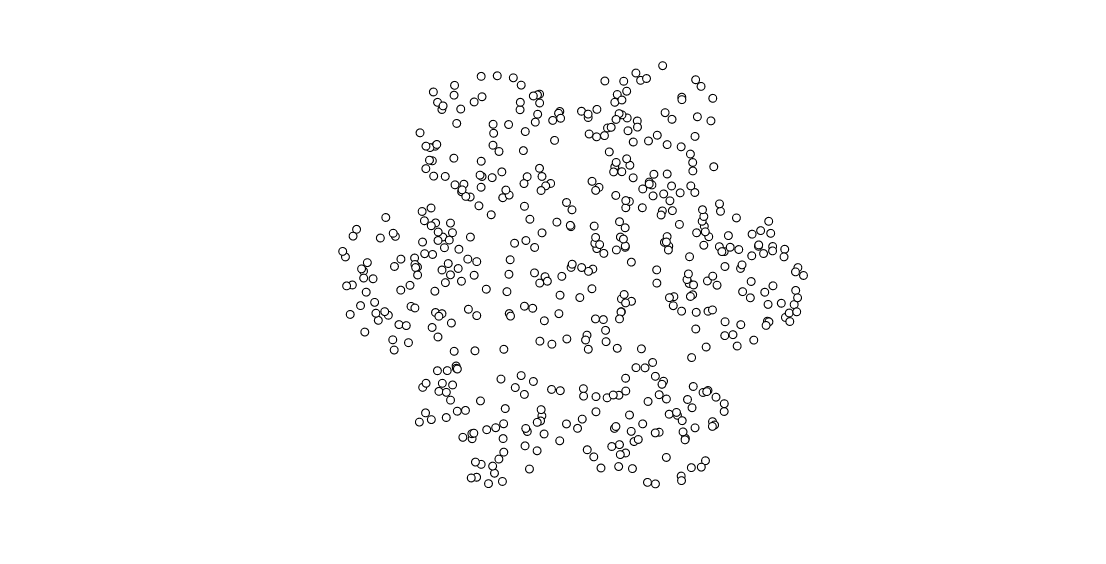
\includegraphics[height=180pt, keepaspectratio = true]{images/k_means_k}  
%	\end{figure}
\end{frame}

\section{Устранение недостатков}

\begin{frame}{Устранение недостатков}
	\begin{itemize}
		\item[--] Несколько случайных кластеризаций
		\item[--] Постепенное наращивание числа $k$
		\item[--] Использование k-means++
	\end{itemize}
\end{frame}

\begin{frame}{k-means++}
	\begin{itemize}
		\item[--] Выбрать первый центроид случайным образом
		\item[--] Для каждой точки найти значение квадрата расстояния до ближайшего центроида.
		\item[--] Выбрать из этих точек следующий центроид так, чтобы вероятность выбора точки была пропорциональна вычисленному для неё квадрату расстояния
	\end{itemize}
\end{frame}

\begin{frame}{X-means}
	\alert{Идея}:\\
	\begin{itemize}
		\item[--] Получать на вход не k, а диапазон, в котором может находиться k.
		\item[--] Запустить k-means на самом маленьком значении из диапазона.
		\item[--] Разбивать пополам полученные кластеры и проверять, не улучшилась ли кластеризация.
	\end{itemize}
\end{frame}

\begin{frame}{X-means}
\TODO{картинка}
%	\begin{figure}[htbp]
%	  \includegraphics[height=140pt, keepaspectratio = true]{images/x-means}  
%	    \includegraphics[height=140pt, keepaspectratio = true]{images/x-means-1}
%	\end{figure}
\end{frame}

\begin{frame}{X-means}
  \centering  
  Как проверить, что кластеризация улучшилась?
\end{frame}

\begin{frame}{Байесовский информационный критерий}
	$BIC_j = L_j(X)  + \frac{d}{2} \log(n)$\\
	\bigbreak
	$L_j$ -- логарифмическая функция правдоподобия для $j$-й модели \\
	$d$ -- длина вектора параметров\\
	$n$ -- количество объектов в выборке\\
\end{frame}

\section{Недостатки k-means}

\begin{frame}{"Не сферические данные"}
  \TODO{картинка}
%	\begin{figure}[htbp]
%	  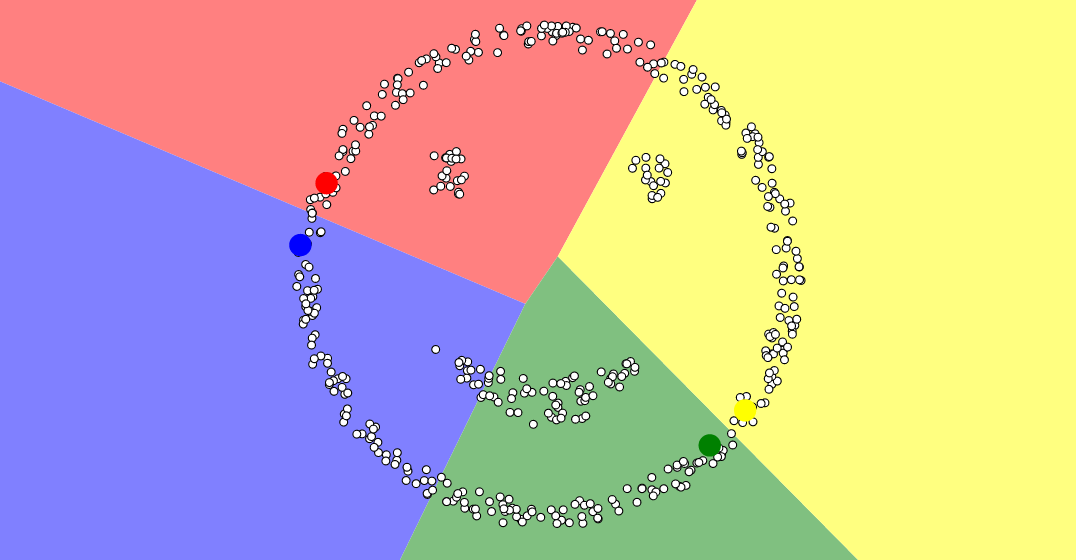
\includegraphics[height=180pt, keepaspectratio = true]{images/non_spherical-1}  
%	\end{figure}
\end{frame}	

\begin{frame}{"Не сферические данные"}
	\TODO{картинка}
%	\begin{figure}[htbp]
%	  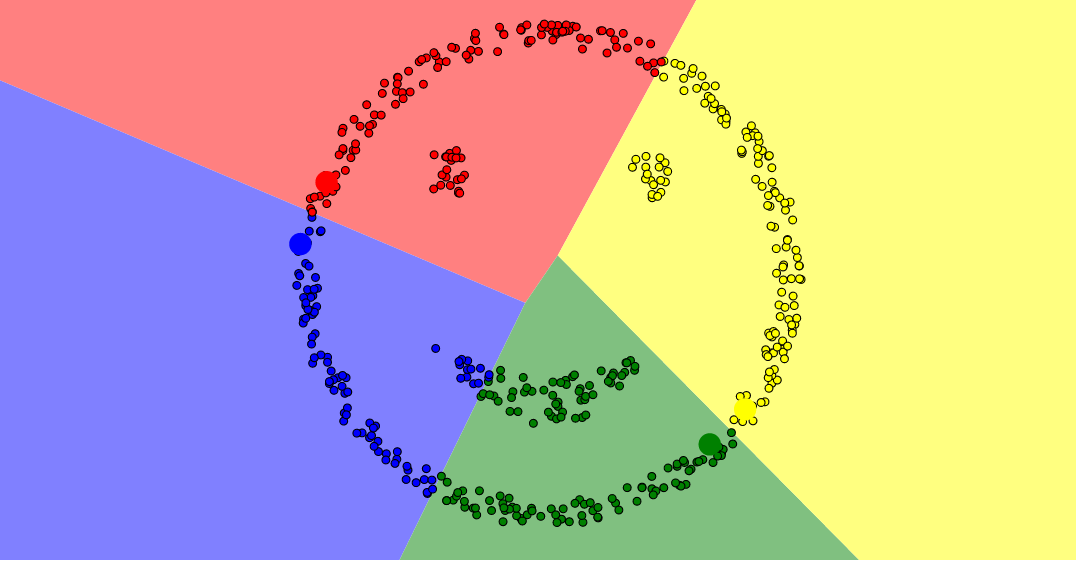
\includegraphics[height=180pt, keepaspectratio = true]{images/non_spherical-2}  
%	\end{figure}
\end{frame}

\begin{frame}{Разноразмерные кластеры}
\TODO{картинка}
%	\begin{figure}[htbp]
%	  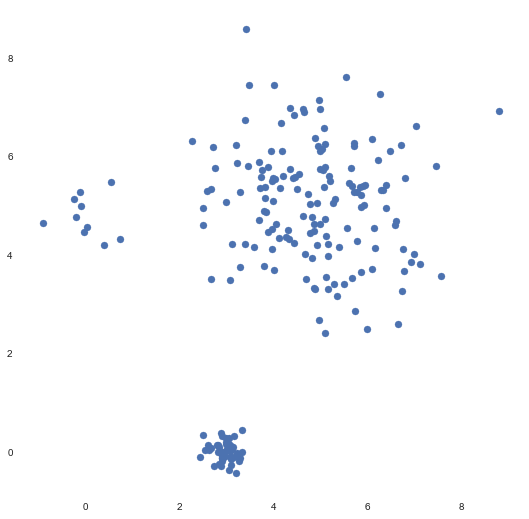
\includegraphics[height=180pt, keepaspectratio = true]{images/different_sizes-1}  
%	\end{figure}
\end{frame}

\begin{frame}{Разноразмерные кластеры}
\TODO{картинка}
%	\begin{figure}[htbp]
%	  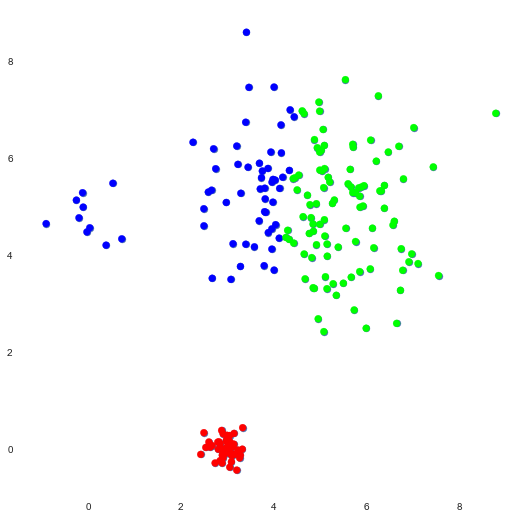
\includegraphics[height=180pt, keepaspectratio = true]{images/different_sizes-2}  
%	\end{figure}
\end{frame}

\begin{frame}[standout]
  Вопросы?
\end{frame}

\appendix

\begin{frame}{На следующей лекции}
  \TODO{what next}
\end{frame}

\end{document}